\section{O artefato GP-PME}
\label{sec:artefato}

\subsection{Visão geral e princípio de contingência}

O GP-PME organiza uma jornada de governança e gestão de TI para empresas nas quais o proprietário, um responsável de TI e poucos colaboradores acumulam funções. Sua unidade básica não é o processo formal, mas um ciclo verificável de decisão: uma necessidade de negócio ou risco entra no sistema; é classificada segundo valor, urgência e capacidade; recebe um responsável e um limite de execução; produz um artefato curto; e retorna ao ponto de governança por meio de uma métrica ou evidência.

O princípio de contingência aparece em três escolhas. Primeiro, a quantidade de mecanismos ativos depende da maturidade e da dor dominante. Segundo, cada prática possui uma forma manual, evitando que automação seja requisito de entrada. Terceiro, a expansão só ocorre depois que a organização consegue sustentar a rotina anterior com evidências. O modelo não procura ``implantar um framework completo'', mas compor o menor sistema coerente para a situação observada.

\begin{figure}[H]
  \centering
  \IfFileExists{figures/generated/gppme-architecture.pdf}{%
    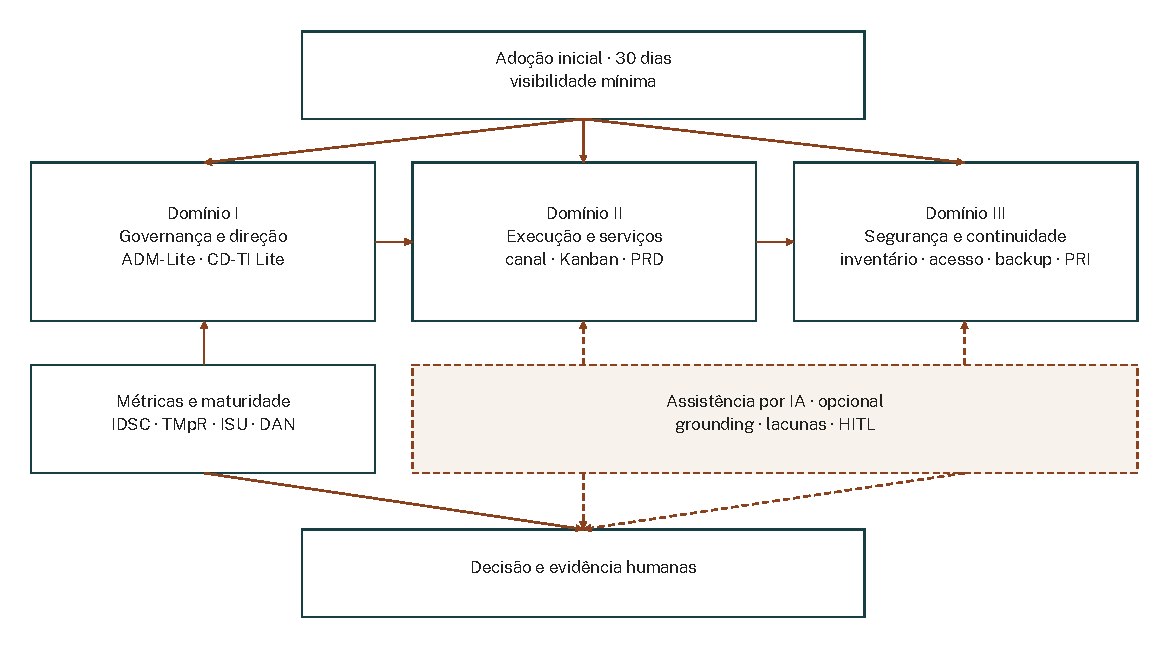
\includegraphics[width=\textwidth]{figures/generated/gppme-architecture.pdf}%
  }{%
    \fbox{\parbox{0.92\textwidth}{\centering
      Fase Zero $\rightarrow$ Governança Essencial $\leftrightarrow$ Execução Ágil $\leftrightarrow$ Segurança Crítica; métricas e maturidade atravessam os três pilares; assistência por IA é opcional e permanece sob HITL.}}
  }
  \caption{Arquitetura conceitual do GP-PME. As setas representam ciclos de informação e decisão, não uma sequência rígida.}
  \label{fig:arquitetura-gppme}
\end{figure}

\subsection{Porta de entrada: diagnóstico e Fase Zero}

O diagnóstico inicial usa dez perguntas binárias, cada resposta positiva condicionada à apresentação de uma evidência. Na versão corrente do artefato, a soma forma o Índice de Maturidade da TI (IM-TI), associado a cinco níveis: 0 (caótico), 1 (organizado reativo), 2 (governança básica), 3 (inovação incremental) e 4 (governança adaptativa). A função do índice é orientar a próxima ação e não certificar conformidade.

A Fase Zero dura 30 dias e estabelece condições mínimas de observação. Na primeira semana, cria-se um canal único de demanda e um quadro Kanban. Na segunda, consolidam-se uma base curta de conhecimento, o inventário de ativos críticos e a situação dos backups. Na terceira, prepara-se um Plano de Resposta a Incidentes (PRI) e inicia-se o CD-TI Lite. Na quarta, publicam-se três indicadores visíveis e o diagnóstico é repetido. Metas sugeridas nesse roteiro são objetivos de desenho; até a execução do protocolo, não constituem resultados médios esperados.

\subsection{Pilar I: Governança Essencial}

O primeiro pilar traduz o ciclo de avaliar, direcionar e monitorar em ADM-Lite. Seu principal ritual é o CD-TI Lite, reunião quinzenal de 30 minutos entre a direção e o responsável por TI. A pauta reserva cinco minutos para indicadores, quinze para alinhamento e priorização, cinco para riscos e dívida técnica e cinco para decisões e responsáveis. A saída é uma ata de uma página, suficiente para registrar o que foi decidido, por quem e com qual evidência de acompanhamento.

A Matriz de Quatro Quadrantes conecta cada iniciativa a uma finalidade de negócio: geração de receita, redução de custos, experiência de cliente ou colaborador, e resiliência ou segurança. O RACI-Lite explicita quem executa, aprova, é consultado e informado, admitindo acumulação de papéis, mas não ausência de responsabilidade. Quando uma iniciativa não encontra vínculo com um quadrante, responsável ou métrica, ela retorna à fila para refinamento.

\subsection{Pilar II: Execução Ágil}

O segundo pilar combina práticas de fluxo e ciclos curtos. Todas as demandas entram por um canal único e percorrem um quadro com quatro estados: A Fazer, Em Andamento, Em Teste e Concluído. O limite padrão de trabalho em progresso é três por executor. O objetivo é tornar filas e bloqueios observáveis, não reproduzir uma implementação integral de Scrum ou ITIL.

A cadência mínima inclui planejamento semanal de quinze minutos, verificação diária de cinco minutos e retrospectiva de quinze minutos. Incidentes críticos usam uma raia de expedite e suspendem explicitamente uma tarefa de menor prioridade, evitando que ``urgente'' signifique trabalho adicional invisível. Demandas de desenvolvimento são reduzidas a um MVP de até duas semanas e documentadas em PRD curto com dor, histórias, critérios verificáveis, escopo negativo, requisito não funcional, métrica afetada e aprovação humana.

\subsection{Pilar III: Segurança Crítica}

O terceiro pilar seleciona controles de maior efeito operacional imediato. O Inventário 80/20 registra os ativos cuja indisponibilidade ou comprometimento afeta a maior parte da operação. Identidade e acesso são tratados por contas individuais, autenticação multifator em sistemas críticos e privilégio mínimo. Backups devem ser automáticos e acompanhados de teste periódico de restauração. O PRI de uma página define contenção, comunicação, responsáveis e recuperação.

Um checklist de dez controles amplia essa linha de base conforme a organização amadurece. Cada item recebe estado (implementado, em andamento ou não implementado), evidência, próximo passo, responsável e prazo. A classificação de risco usa probabilidade e impacto em categorias ordinais; quando faltam dados técnicos, o artefato exige registro da lacuna ou auditoria local, em vez de inferência automática.

\subsection{Métricas transversais}

Três indicadores formam o painel operacional inicial. O Índice de Disponibilidade de Serviços Críticos (IDSC) é dado por
\begin{equation}
  \mathrm{IDSC}=\frac{T_{\text{previsto}}-T_{\text{indisponível}}}{T_{\text{previsto}}}\times 100.
\end{equation}
O Tempo Médio para Resolução (TMpR) é a soma das durações dos chamados encerrados dividida pela quantidade de chamados. O Índice de Satisfação do Usuário (ISU) é a média das notas coletadas no período. Os três valores são discutidos em conjunto, pois disponibilidade alta pode coexistir com resolução lenta ou experiência ruim.

Para decisões de modernização, a Dívida de Arquitetura Normalizada (DAN) relaciona o esforço estimado de refatoração ao orçamento anual de TI:
\begin{equation}
  \mathrm{DAN}=\frac{H_{\text{refatoração}}\times C_{\text{hora}}}{O_{\text{TI, anual}}}.
\end{equation}
O Custo de Oportunidade Tecnológica (COT) consolida custos diretos e indiretos de uma mudança, e o retorno projetado é calculado a partir de premissas registradas. DAN, COT e ROI são instrumentos de decisão e análise de sensibilidade; valores produzidos por cenários não devem ser tratados como retorno observado.

\subsection{Camada opcional de assistência por IA}

A IA é uma camada transversal e opcional. No modo manual, todos os rituais e artefatos podem ser executados com reunião, planilha, quadro e templates. No modo assistido, agentes especializados ajudam a fazer triagem, gerar uma primeira minuta, calcular métricas, recuperar trechos da base de conhecimento e auditar requisitos. A decisão de priorizar, aprovar, alterar acesso, conter incidente ou investir permanece com uma pessoa identificada.

O protocolo de segurança epistêmica possui quatro regras. A saída deve estar ancorada em dados fornecidos ou em fonte recuperada; informações ausentes recebem o marcador de dado insuficiente; cálculos determinísticos são separados de narrativa gerada; e qualquer artefato com efeito organizacional passa por Human-in-the-Loop (HITL). Essa arquitetura procura capturar benefícios de assistência sem converter fluência textual em autoridade decisória.

\subsection{Instanciação computacional}

A versão analisada no repositório \citep{gppme2026repo} instancia o artefato em guias, templates, oito skills, nove agentes prontos, um orquestrador com oito especialistas, cinco adaptadores de plataformas de trabalho, busca textual/semântica, grafo de conhecimento e serviços de API/MCP. Regras como IM-TI, indicadores, DAN, COT e ROI também possuem implementações determinísticas. Esses componentes ampliam os canais de uso do mesmo núcleo de conhecimento; não adicionam novos pilares conceituais.

Alguns documentos históricos chamam a assistência por IA de ``Pilar IV''. Para manter coerência com a hipótese original e com o requisito de funcionamento manual, este artigo adota a nomenclatura ``três pilares essenciais mais uma camada opcional''. A diferença é semântica e arquitetural: uma prática opcional não pode ser condição para que o núcleo do framework seja considerado completo.
